%%%%%%%%%%%%%%%%%%%%%%%%%%%%%%%%%%%%%%%%%
% Student: Francis Pruter
% Assignment 2
% CS 595
%
% used the template from:
% http://www.latextemplates.com/template/structured-general-purpose-assignment
%%%%%%%%%%%%%%%%%%%%%%%%%%%%%%%%%%%%%%%%%

%----------------------------------------------------------------------------------------
%	PACKAGES AND OTHER DOCUMENT CONFIGURATIONS
%----------------------------------------------------------------------------------------

\documentclass{article}
\setlength{\paperheight}{11in}

\usepackage{fancyhdr} % Required for custom headers
\usepackage{lastpage} % Required to determine the last page for the footer
\usepackage{extramarks} % Required for headers and footers
\usepackage{graphicx} % Required to insert images
\usepackage{listings} % Required to insert codes
\usepackage{pdfpages}

% Margins
\topmargin=-0.45in
\evensidemargin=0in
\oddsidemargin=0in
\textwidth=6.5in
\textheight=9.0in
\headsep=0.25in 

\linespread{1.1} % Line spacing

% Set up the header and footer
\pagestyle{fancy}
\lhead{\hmwkAuthorName} % Top left header
\chead{\hmwkClass\ (\hmwkClassInstructor\ \hmwkClassTime): \hmwkTitle} % Top center header
\rhead{\firstxmark} % Top right header
\lfoot{\lastxmark} % Bottom left footer
\cfoot{} % Bottom center footer
\rfoot{Page\ \thepage\ of\ \pageref{LastPage}} % Bottom right footer
\renewcommand\headrulewidth{0.4pt} % Size of the header rule
\renewcommand\footrulewidth{0.4pt} % Size of the footer rule

\setlength\parindent{0pt} % Removes all indentation from paragraphs

   
%----------------------------------------------------------------------------------------
%	NAME AND CLASS SECTION
%----------------------------------------------------------------------------------------

\newcommand{\hmwkTitle}{Assignment\ \#1} % Assignment title
\newcommand{\hmwkDueDate}{Thursday,\ September\ 11,\ 2014} % Due date
\newcommand{\hmwkClass}{CS\ 595} % Course/class
\newcommand{\hmwkClassTime}{04:20pm} % Class/lecture time
\newcommand{\hmwkClassInstructor}{MLN} % Teacher/lecturer
\newcommand{\hmwkAuthorName}{Francis W. Pruter, Jr.} % Your name

\begin{document}    



% Start your text
\section{Problem 1:}
\label{Problem 1}

{\bf 1.  Write a Python program that extracts 1000 unique links fromTwitter.  
\newline\newline
Also note that you need to verify that the final target URI (i.e., the one that responds with a 200) is unique.  You could have different shortened URIs for www.cnn.com.  \newline
For example, 
\newline
http://cnn.it/1cTNZ3V\newline
http://t.co/BiYdsGotTd\newline
} 

{\it Below is the Python coded used to extract 1000 unique URIs and ensure the links are valid and unique.\newline
I used an adapted code from Craig Addyman (http://www.craigaddyman.com/mining-all-tweets-with-python/)
\newline
I've included a the uniqueURI file in the githubb
\newline\newline

}

\lstinputlisting[language=Python,numbers=left, frame=single,caption=extractTwitter.py, label={extractTwitter.py}, breaklines=true,
morekeywords={models, lambda, forms}]{extractTwitter.py}


\newpage
\section{Problem 2:}
\label{Problem 2}

{\bf Download the TimeMaps for each of the target URIs.  We'll use the mementoweb.org \newline
Aggregator, so for example:\newline\newline

URI-R = http://www.cs.odu.edu/
\newline
URI-T = http://mementoweb.org/timemap/link/http://www.cs.odu.edu/
\newline
You could use the cs.odu.edu aggregator:
\newline
URI-T = http://mementoproxy.cs.odu.edu/aggr/timemap/link/1/http://www.cs.odu.edu/
\newline\newline
But be sure to say which aggregator you use -- they are likely to give different answers.
\newline
Create a histogram of URIs vs. number of Mementos (as computed from the TimeMaps).  For example, 100 URIs with 0 Mementos, 300 URIs with 1 Memento, 400 URIs with 2 Mementos, etc.
\newline\newline
See: http://en.wikipedia.org/wiki/Histogram
\newline
Note that the TimeMaps can span multiple pages.  
\newline\newline
} 

{\it I used two Bash scripts to solve this problem. \newline\newline
The first one downloads the TimeMaps for each URI using memento.web.org.  It will also check to see if if there is a next page and extract the data from that page as well.  
\newline
}

\lstinputlisting[language=Bash,numbers=left, frame=single,caption=getMementos.py, label={getMementos}, breaklines=true,
morekeywords={models, lambda, forms}]{getMementos.txt}

{\it 
The second one uses ``grep" to find each line with mementos in it and uses ``wc -l'' to count each line for the number of occurances.  
\newline
}

\lstinputlisting[language=Bash,numbers=left, frame=single,caption=numMementos.py, label={numMementos}, breaklines=true,
morekeywords={models, lambda, forms}]{numMementos.txt}


\begin{figure}[h!]
    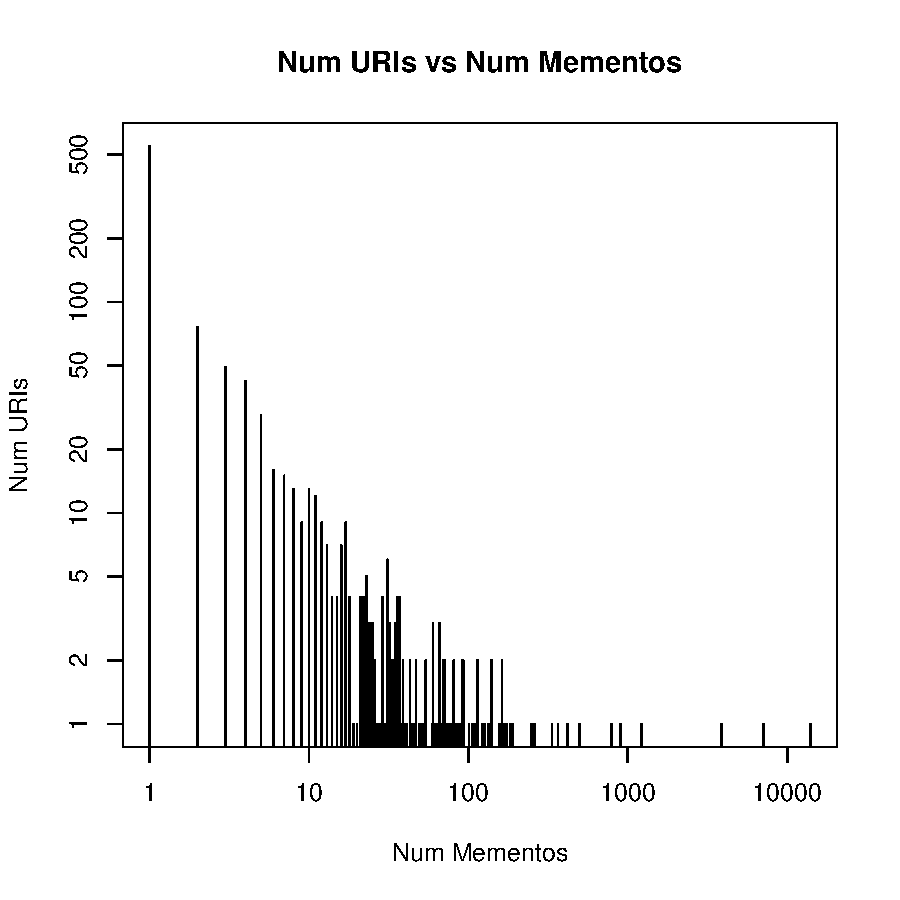
\includegraphics[width=\textwidth]{prob2}
    \caption{Above is a histograph: URIs vs. number of Mementos.  I had to use a log log scale to shore the relationship between the two.  This shows that most URI have a few mementos.  This appears to be because twitter is a social media site and in this case Tim O'Reilly was posting recent websites.  The website with the more mementos was www.healthcare.gov}
\end{figure}


\newpage
\section{Problem 3:}
\label{Problem 3}

{\bf Estimate the age of each of the 1000 URIs using the ``Carbon Date'' tool:
\newline\newline
http://ws-dl.blogspot.com/2013/04/2013-04-19-carbon-dating-web.html
\newline\newline
Note: you'll have better luck downloading and installing the tool rather than using the web service (which will run slowly and likely be unreliable).
\newline\newline
For URIs that have more than 0 Mementos and an estimated creation date, create a graph with age (in days) on one axis and number of mementos on the other.
\newline
\newline


}
{\it 
This was probably the hardest part of the assignment.  Not the problem itself, but executing.  I ended up modifying the local.py to add threading and executed 10 links at a time.  This reduced run time from 12+ hours to about 45 minutes  Below is the modified code.  
}

\lstinputlisting[language=Python,numbers=left, frame=single,caption=local.py, label={local}, breaklines=true,
morekeywords={models, lambda, forms}]{local.py}

{\it 
The next part I used python to print the estimated days alive per link based on the estimated creation date from local.py.  Sites without an estimated creation date are listed as ``0''
}

\lstinputlisting[language=Python,numbers=left, frame=single,caption=creationdate.py, label={creationdat}, breaklines=true,
morekeywords={models, lambda, forms}]{creationdate.py}



\begin{figure}[h!]
    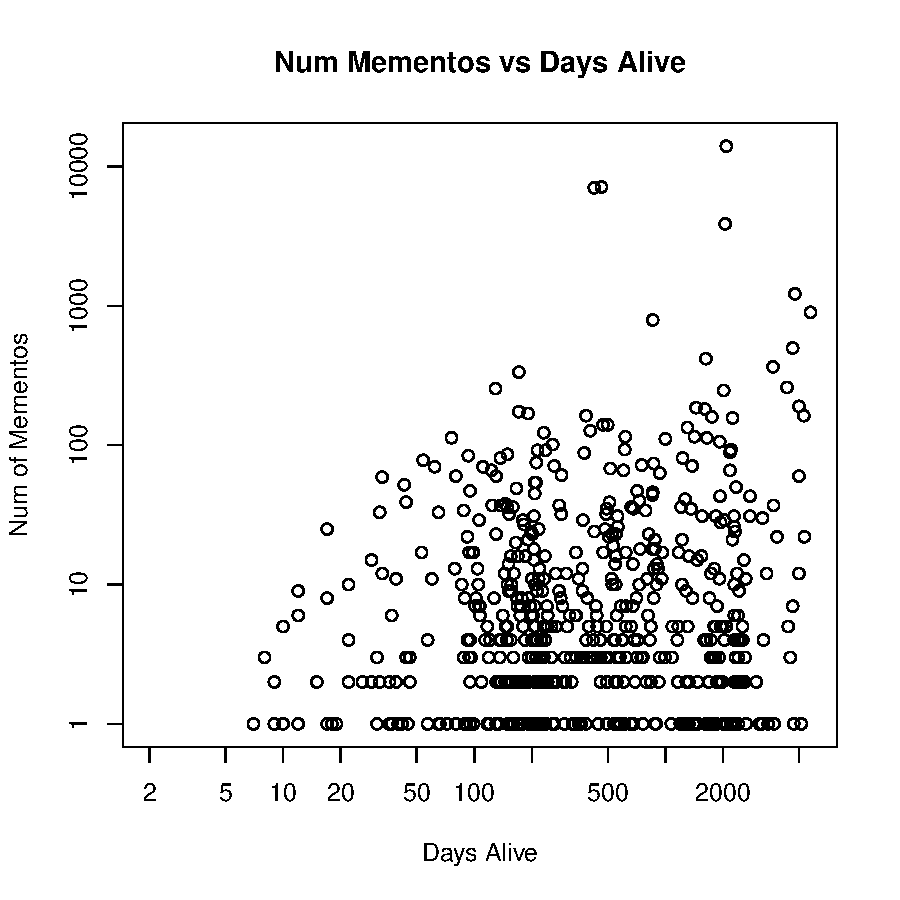
\includegraphics[width=\textwidth]{prob3}
    \caption{Above is a plot to show the relations between the nmber of mementos vs days alive.  Again, in order to see the relationship, I had to use a log-log scale.  As expected, the longer ago the website was created the more mementos were created.}
\end{figure}


 
% Stop your text
\end{document}